\documentclass[tikz]{standalone}
\usepackage{pgfplots}
\usepackage{mathptmx}
\usepackage{ctex}
% \pgfplotsset{compat=1.16}
\begin{document}
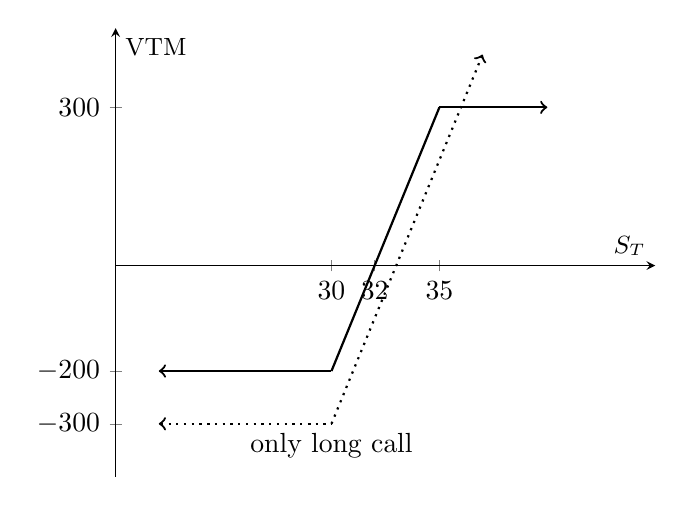
\begin{tikzpicture}
    \begin{axis}[
        axis lines = middle,
        xlabel = {$S_T$},
        ylabel = {VTM},
        ymin=-400, ymax=450,
        xmin=20, xmax=45,
        xtick={30,32,35},
        ytick={-300,-200,0,300},
        % width=10cm,
        % height=7cm,
        % axis equal,
        label style={font=\small}
    ]
    % 定义参数
    \def\Ka{30} % 执行价格
    \def\Kb{35} % 执行价格
    \def\Pa{3}  % 期权费
    \def\Pb{1}  % 期权费
    
    % 绘制看涨期权到期收益曲线
    \addplot[domain=22:\Ka,<-,thick] {(-\Pa+\Pb)*100};
    \addplot[domain=\Ka:\Kb,thick] {(x-\Ka-\Pa+\Pb)*100};
    \addplot[domain=\Kb:40, ->,thick] {(\Kb-\Ka+\Pb-\Pa)*100};

    \addplot[domain=22:\Ka,<-, dotted,thick]{-\Pa*100};
    \addplot[domain=\Ka:37,->, dotted,thick]{(x-\Ka-\Pa)*100};

    % \addplot[domain=\Kb:14300, dashed] {x - \Kb - \Pb};
    % \addplot[domain=13600:\Ka, dashed] {x + \Pa - \Ka};
    % \addplot[domain=\Ka:14300, dashed] {\Pa};

    % \addplot[domain=13600:\Ka, thick, green] {x + \Pa - \Ka - \Pb};
    % \addplot[domain=\Ka:\Kb, thick, green] {-32};
    % \addplot[domain=\Kb:14032, thick, green] {x - \Kb - \Pb + \Pa};
    % \addplot[domain=14032:14300, thick, red] {x - \Kb - \Pb + \Pa};

    % \addplot[domain=13600:14300] {0};

    % \addplot[dashed] coordinates {(\Ka,0) (\Ka,\Pa)};
    % \addplot[dashed] coordinates {(\Kb,0) (\Kb,-\Pb)};
    
    % 标记执行价格和盈亏平衡点
    % \addplot[dashed, domain=0:150] coordinates {(\Ka,-50) (\Ka,150)};
    % \addplot[dashed, domain=0:150] coordinates {(\Ka+\P,-50) (\Ka+\P,150)};
    
    % % 添加标签
    % \node at (axis \Ka,-\Pa*100) [below] {only long call};
    % \node at (axis cs:150,50) [right] {Profit = $S_T - Ka - P$};
    
    % 标记执行价格和盈亏平衡点
    \node at (axis cs:\Ka,-\Pa*100) [below] {only long call};
    % \node at (axis cs:\Ka-\Pa,0) [below left] {$13729$};

    % \node at (axis cs:\Kb,-\Pb) [right] {$-\Pb$};
    % \node at (axis cs:\Kb+\Pb,0) [below right] {$14103$};
    
    \end{axis}
\end{tikzpicture}

\end{document}